\section*{Sistemas de numeração II}


\frame{
	\frametitle{Sistemas de numeração}
	\begin{block}{Sistema octal}
		\begin{itemize}
			\item Caracteres 0 a 7.
			\item CLP - gerenciamento de memórias.
			\item Novamente... notação posicional.
			\item Quantidade de dígitos para representar um número.
		\end{itemize}
	\end{block}

	\centerline{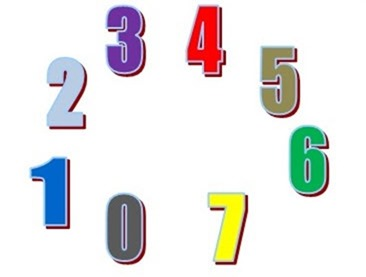
\includegraphics[width=0.4\linewidth]{Figuras/Ch2/octal.jpg}}
}

\frame{
	\frametitle{Sistemas de numeração}
	\begin{block}{Sistema hexadecimal}
		\begin{itemize}
			\item 16 caracteres... e agora, como representar?
			\item Novamente... notação posicional.
			\item Quantidade de dígitos para representar um número.
			\item Aplicações computacionais.
		\end{itemize}
	\end{block}

	\bigskip

	\centerline{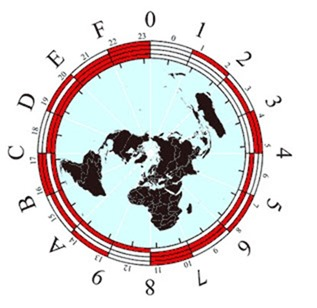
\includegraphics[width=0.37\linewidth]{Figuras/Ch2/hexa.jpg}}
}

\section*{Conversão entre bases numéricas II}

\frame{
	\frametitle{Conversão octal-decimal}
	\begin{block}{Procedimento}
		\begin{itemize}
			\item Se dá pela soma das multiplicações de cada termo por sua potência de base 8 equivalente. 
		\end{itemize}
	
		\bigskip
	
		\begin{minipage}{0.49\linewidth}
			\centering
			\ConvertFromBase{8}{331}
		\end{minipage}
		\hfill
		\begin{minipage}{0.49\linewidth}
			\centering
			\ConvertFromBase{8}{45}
		\end{minipage}
	\end{block}
%	\centerline{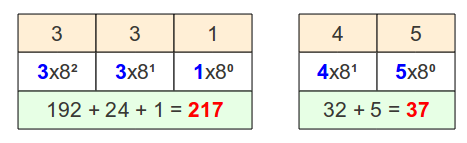
\includegraphics[width=0.8\linewidth]{Figuras/Ch2/octaldec.png}}
}


\frame{
	\frametitle{Conversão decimal-octal}
	\begin{block}{Procedimento}
		\begin{itemize}
			\item Método das divisões sucessivas 
		\end{itemize}
		
		\vspace{0.5cm}
	
		\centering
		\begin{tabular}{c}
			\basetenconversiontable{157}{8}
		\end{tabular}
	\end{block}

	
%	\centerline{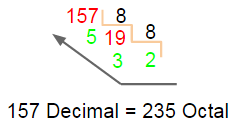
\includegraphics[width=0.6\linewidth]{Figuras/Ch2/decoctal.png}}
}

\frame{
	\frametitle{Conversão hexadecimal-decimal}
	\begin{block}{Procedimento}
		\begin{itemize}
			\item Se dá pela soma das multiplicações de cada termo por sua potência de base 16 equivalente. 
		\end{itemize}
	
		\bigskip
		
		\centering
		\ConvertFromBase{16}{A3}
	\end{block}
%	\centerline{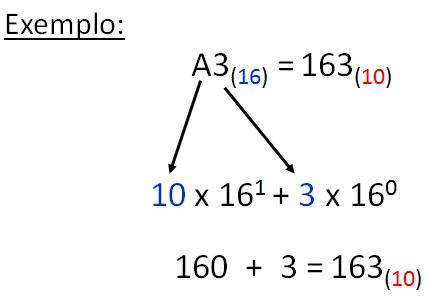
\includegraphics[width=0.5\linewidth]{Figuras/Ch2/hexadec.jpg}}
}


\frame{
	\frametitle{Conversão decimal-hexadecimal}
	\begin{block}{Procedimento}
		\begin{itemize}
			\item Método das divisões sucessivas 
		\end{itemize}
	
		\vspace{0.5cm}
		
		\centering
		\begin{tabular}{c}
			\basetenconversiontable{12412}{16}
		\end{tabular}
	\end{block}
	
%	\centerline{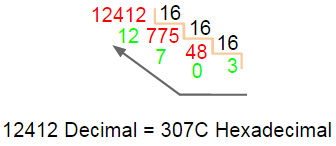
\includegraphics[width=0.7\linewidth]{Figuras/Ch2/dechexa.png}}
}

\section*{Resumo}
\frame{
	\frametitle{O que vimos até agora?}
	\begin{block}{}
		Até agora o "centro das atenções" era o sistema \textbf{DECIMAL}
		\begin{itemize}
			\item decimal-binário-decimal
			\item decimal-octal-decimal
			\item decimal-hexadecimal-decimal
		\end{itemize}
	\end{block}
	
	\centering
	\begin{tikzpicture}[node distance=1cm, base/.style={
		% The shape:
		rectangle,minimum size=6mm,rounded corners=3mm,
		% The rest
		very thick,draw=black!50,
		fill=black!20}]
	
	\matrix (m) [matrix of nodes,row sep=1cm,column sep=1cm,ampersand replacement=\&] {
		|[base] (dec)| Decimal \& |[base] (oct)| Octal \\
		|[base] (bin)| Binário \& |[base] (hex)| Hexadecimal \\
	};

	\graph {(dec) <-> (oct); (dec) <-> (bin); (dec) <-> (hex);};
		
	\end{tikzpicture}
%	\centerline{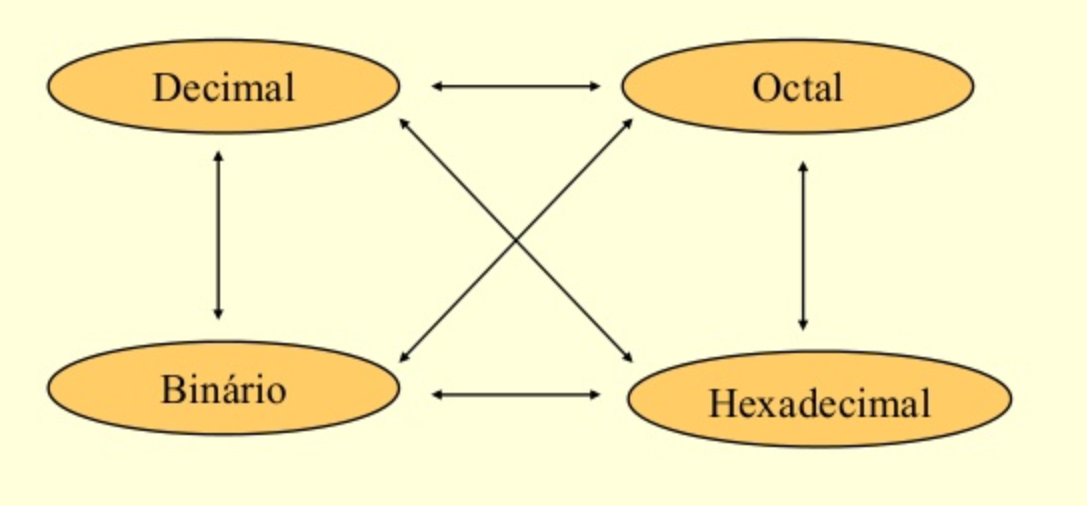
\includegraphics[width=0.5\linewidth]{Figuras/Ch2/resumo.PNG}}
	
	\begin{block}{}
		\textbf{E como converter entre as outras bases?}
	\end{block}
}

\section*{Conversão entre bases numéricas III}
\frame{
	\frametitle{Conversão binário-octal}
	\begin{block}{Procedimento}
		\begin{itemize}
			\item Basta separar em grupos de \textbf{3 bits} a partir da direita 
		\end{itemize}
	
		\vspace{0.5cm}
		
		\centering
		\begin{tikzpicture}
		
		\matrix (m) [matrix of math nodes,row sep=1cm,column sep=2pt,ampersand replacement=\&] {
			|(g1)| \underbrace{100} \&[0.2cm] \& |(g2)| \underbrace{001} \&[0.2cm] \& |(g3)| \underbrace{111} \\
			\& 		\& |(r)| \; 4\ 1\ 7_2	\& 		\& \\
		};
		
		\node[xshift=-3em,yshift=-1.02em] at (m.north west) {$ \num{100001111}_8= $};
		
		\draw[-Latex,thick] ($ (g1)+(0pt,-7pt) $) -- ($ (r.north)+(-9pt,0) $);
		\draw[-Latex,thick] ($ (g2)+(0,-7pt) $) -- ($ (r.north)+(-1pt,0) $);
		\draw[-Latex,thick] ($ (g3)+(0pt,-7pt) $) -- ($ (r.north)+(8pt,0) $);
		
		\end{tikzpicture}
	\end{block}
%	\centerline{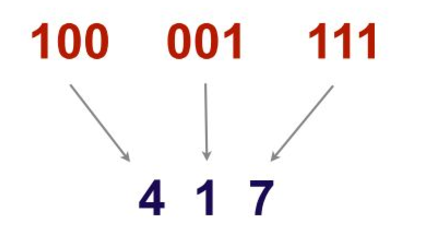
\includegraphics[width=0.5\linewidth]{Figuras/Ch2/binoctal.PNG}}
}

\frame{
	\frametitle{Conversão binário-hexadecimal}
	\begin{block}{Procedimento}
		\begin{itemize}
			\item Basta separar em grupos de \textbf{4 bits} a partir da direita 
		\end{itemize}
	
		\vspace{0.5cm}
		
		\centering
		\begin{tikzpicture}
		
		\matrix (m) [matrix of math nodes,row sep=1cm,column sep=2pt,ampersand replacement=\&] {
			|(g1)| \underbrace{\ \ 11} \&[0.2cm] \& |(g2)| \underbrace{1010} \&[0.2cm] \& |(g3)| \underbrace{0110} \\
			\& 		\& |(r)| \;\ \! 3\ A\ 6_{16}	\& 		\& \\
		};
		
		\node[xshift=-3.5em,yshift=-1.02em] at (m.north west) {$ 11\ \! 1010\ \! 0110_2= $};
		
		\draw[-Latex,thick] ($ (g1)+(0pt,-7pt) $) -- ($ (r.north)+(-12pt,0) $);
		\draw[-Latex,thick] ($ (g2)+(0,-7pt) $) -- ($ (r.north)+(0pt,0) $);
		\draw[-Latex,thick] ($ (g3)+(0pt,-7pt) $) -- ($ (r.north)+(8pt,0) $);
		
		\end{tikzpicture}
	\end{block}
%	\centerline{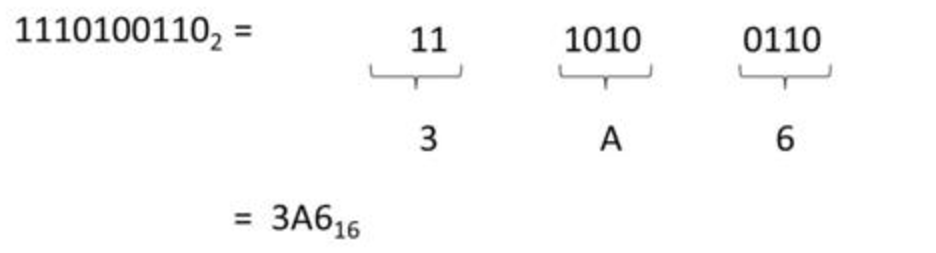
\includegraphics[width=0.9\linewidth]{Figuras/Ch2/binhexa.PNG}}
}

\frame{
	\frametitle{Conversão octal-binário}
	\begin{block}{Procedimento}
		\begin{itemize}
			\item Observe cada dígito e transforme para binário 
		\end{itemize}
	
		\vspace{0.5cm}
		
		\centering
%		\renewcommand{\arraystretch}{1.2}
		\resizebox{\textwidth}{!}{
			\begin{tabular}{lcccc}
				\toprule
				Octal & 4 & 5 & 3 & 6 \\\midrule
				Binário & 100 & 101 & 011 & 110 \\\midrule
				Final & \multicolumn{4}{c}{\num{100101011110}} \\ \bottomrule
		\end{tabular}}
	\end{block}
%	\centerline{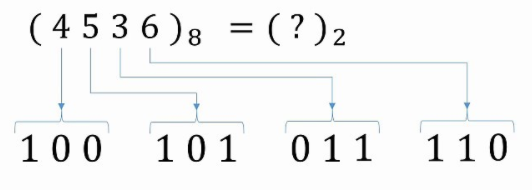
\includegraphics[width=0.6\linewidth]{Figuras/Ch2/octalbin.PNG}}
}

\frame{
	\frametitle{Conversão hexadecimal-binário}
	\begin{block}{Procedimento}
		\begin{itemize}
			\item Observe cada dígito e transforme para binário 
		\end{itemize}
	
		\vspace{0.5cm}
		
		\centering
%		\renewcommand{\arraystretch}{1.2}
		\resizebox{\textwidth}{!}{
			\begin{tabular}{lcccc}
				\toprule
				Hexadecimal & 1 & A & $ 6 $ & 0 \\\midrule
				Binário & 0001 & 1010 & 0110 & 0000 \\\midrule
				Final & \multicolumn{4}{c}{$ 0001\ \! 1010\ \! 0110\ \! 0000 $} \\ \bottomrule
		\end{tabular}}s
	\end{block}
%	\centerline{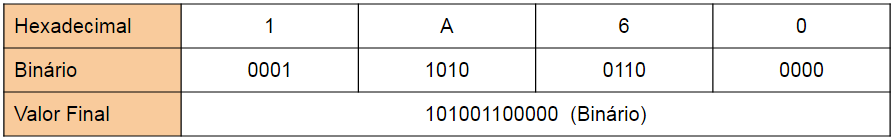
\includegraphics[width=1.1\linewidth]{Figuras/Ch2/hexabin.png}}
}

\frame{
	\frametitle{E as outras duas conversões?}
	\begin{block}{}
		Para completar só faltaram os métodos de conversão:
		\begin{itemize}
			\item Octal para hexadecimal
			\item Hexadecimal para octal
		\end{itemize}
	\end{block}

	\centering
	\begin{tikzpicture}[node distance=1cm, base/.style={
		% The shape:
		rectangle,minimum size=6mm,rounded corners=3mm,
		% The rest
		very thick,draw=black!50,
		fill=black!20}]
	
	\matrix (m) [matrix of nodes,row sep=1cm,column sep=1cm,ampersand replacement=\&] {
		|[base] (dec)| Decimal \& |[base] (oct)| Octal \\
		|[base] (bin)| Binário \& |[base] (hex)| Hexadecimal \\
	};
	
	\graph {(dec) <-> (oct); (dec) <-> (bin); (dec) <-> (hex); (bin) <-> (oct); (bin) <-> (hex);};
	
	\draw[<->,dashed] (oct.south) -- node[red,midway] {\xmark} (hex.north);
	
	\end{tikzpicture}
	
	\begin{block}{}
		\textbf{São métodos complicados, portanto, é melhor utilizar conversões intermediárias.}
	\end{block}
}

\section*{Exercícios}


\frame{
	\frametitle{Exercícios}
	\begin{block}{}
		01. Complete a tabela de conversão abaixo:
	\end{block}

	\vspace{0.2cm}
	
	\centering
%	\renewcommand{\arraystretch}{1.2}
	\resizebox{\textwidth}{!}{
	\begin{tabular}{cccc}
		\toprule
		Decimal & Binário & Octal & Hexadecimal \\ \midrule
		$ 33 $	& & & \\ \midrule
		& $ 1110101 $ & & \\ \midrule
		& & $ 703 $ & \\ \midrule
		& & & $ 1AF $ \\ \bottomrule
	\end{tabular}}
%	\centerline{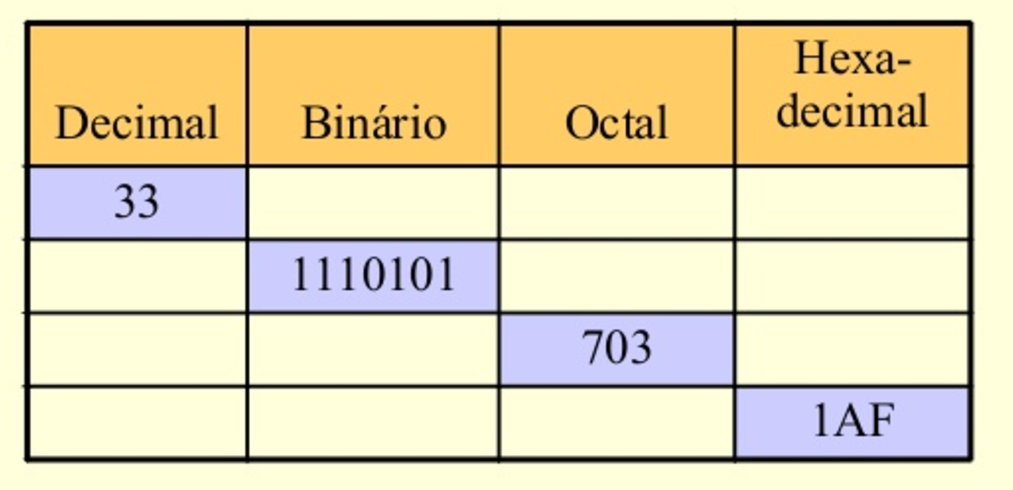
\includegraphics[width=0.8\linewidth]{Figuras/Ch2/exercicio.PNG}}
}

\section*{Referências}

\frame{
	\frametitle{Referências e exercícios complementares}
	\begin{itemize}
		\item IDOETA, Ivan V. e CAPUANO, Francisco G. Elementos de Eletrônica Digital. São Paulo:
		      Editora Érica, ed. 40. 2008.
	\end{itemize}
	\centering{\alert{Página 37 - \textbf{1.6.6 até 1.6.16}}}
}
